\documentclass{article} 
\usepackage{tikz} 
\usetikzlibrary{decorations.pathreplacing}
\usepackage{hyperref}
\usepackage{amsmath} 
\usepackage[a4paper]{geometry}
\usepackage{fancyhdr}
\pagestyle{fancy} 
\lhead{Elektrische Felder}
\rhead{August 2025}
\begin{document}
 
\section{Elektrische Felder}
Ein \emph{elektrisches Feld} ist der Raum um eine elektrische Ladung herum. Es lässt sich durch eine Kraftwirkung auf eine Probeladung erkennen. \newline
Das elektrische Feld wird durch \emph{Feldlinien} veranschaulicht, welche als Pfeil von einer positiven zu einer negativen Ladung, senkrecht zur Oberfläche, gezeichnet werden. Somit stellt die Richtung einer Feldlinie die Kraftrichtung auf freie positive Probeladungen dar. \newline
Quantitativ beschreibt das elektrische Feld die die Kraft pro Ladung, welche auf eine Probeladung wirkt. Somit gilt
\[
 E = \frac{F}{Q}
 \quad \text{in} \quad
 \frac{\text{Newton}}{\text{Coulomn}} 
\] 
 
\subsection{Typische Feldlinien} 
\begin{center}
 \begin{tabular}{c c c}
  homogenes Feld & Dipol & Punktladung \\
  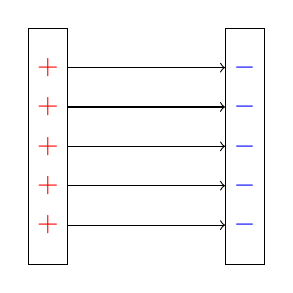
\begin{tikzpicture}
   \draw (0, 3) rectangle (0.5, 0); 
   \draw (2.5, 3) rectangle (3, 0);
   
   \foreach \y in {0.5, 1, 1.5, 2, 2.5} {
     \draw (0.25, \y) node[red] {$+$};
     \draw (2.75, \y) node[blue] {$-$};
     \draw[->] (0.5, \y) -- (2.5, \y);
   } 
  \end{tikzpicture}
  &
  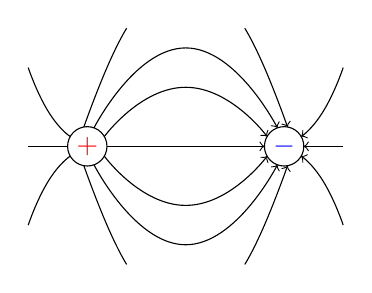
\begin{tikzpicture}
   \draw (0, 0) circle (0.25) node[red] {$+$};
   \draw (2.5, 0) circle (0.25) node[blue] {$-$};
 
   \draw[->] (0.25, 0) -- (2.25,0);  
   \draw[-] (-0.25, 0) -- (-0.75,0);
   \draw[->] (3.25, 0) -- (2.75,0);
  
   \foreach \y in {-1,1} {
    \draw[->] plot [smooth, tension=1] coordinates {({cos(30)*0.25}, {\y*sin(30)*0.25}) (1.25, \y*0.75) ({2.5-cos(30)*0.25}, {\y*sin(30)*0.25})};
    \draw[->] plot [smooth, tension=1] coordinates {({cos(70)*0.25}, {\y*sin(70)*0.25}) (1.25, \y*1.25) ({2.5-cos(70)*0.25}, {\y*sin(70)*0.25})};
 
    \draw plot [smooth, tension=1] coordinates {({cos(100)*0.25}, {\y*sin(100)*0.25}) (0.25, \y*1) (0.5, \y*1.5)};
    \draw[->] plot [smooth, tension=1] coordinates {(2, \y*1.5) (2.25, \y*1) ({2.5-cos(100)*0.25}, {\y*sin(100)*0.25})};
 
    \draw plot [smooth, tension=1] coordinates {({cos(150)*0.25}, {\y*sin(150)*0.25}) (-0.5, \y*0.45) (-0.75, \y*1)};
    \draw[->] plot [smooth, tension=1] coordinates {(3.25, \y*1) (3, \y*0.45) ({2.5-cos(150)*0.25}, {\y*sin(150)*0.25})}; 
   } 
  \end{tikzpicture} 
  &
  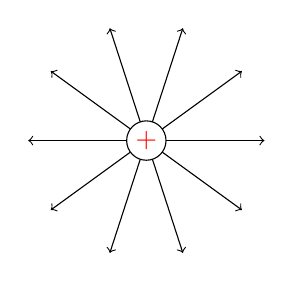
\begin{tikzpicture}
   \draw (0, 0) circle (0.25) node[red] {$+$};
 
   \foreach \id in {0,...,9} {
    \pgfmathsetmacro{\deg}{\id*36}
    \draw[->] ({\deg}:0.25) -- ({\deg}:1.5);
   }  
  \end{tikzpicture}
 \end{tabular} 
\end{center} 
Ein homogenes Feld, wie das Feld zwischen zwei Plattenkondensatoren, wird dadurch gekennzeichnet, dass es überall gleich groß, in die gleiche Richtung zeigend, ist. \newline
Das Feld einer Punktladung wird auch ein radialsymmetrisches Feld gennant. 
 
\subsection{Faradayscher Käfig}
\begin{minipage}{\dimexpr\linewidth-5cm} 
 Innerhalb eines Metallrings zwischen zwei Plattenkondesatoren herrscht ein freies Feld, ohne jeglicher Wirkung einer von Ladung. Dies liegt daran, dass durch die Influenz die Ladungen des Rings auf seine zwei Seiten aufgeteilt werden. Dadurch entsteht ein elektrisches Feld, nur innerhalb des Rings, wessen Feldlinien von der positiv geladenen Seite des Rings, hier rechts, zur negativ geladenene Seite, hier links, gehen würden. {Weil\parfillskip=0pt\par} \vspace{0.1em}
\end{minipage} 
\hfill
\begin{minipage}{5cm}
 \center 
 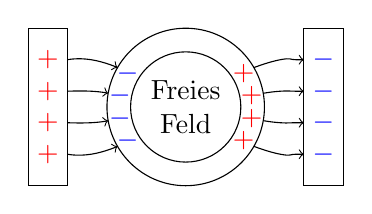
\begin{tikzpicture}
   \draw (0, 2) rectangle (0.5, 0); 
   \draw (3.5, 2) rectangle (4, 0);
   
   \draw (2, 1) circle (0.7) node[align=center] {Freies \\ Feld};
   \draw (2, 1) circle (1);  
  
   \foreach \id in {1,..., 4} { 
    \pgfmathsetmacro{\y}{(\id)*(2/5)}
 
    \draw (0.25, \y) node[red] {$+$};
    \draw (3.75, \y) node[blue] {$-$};
 
    \pgfmathsetmacro{\deg}{-30+(\id-1)*20)}
 
    \draw ({2-cos(\deg)*0.85}, {1+sin(\deg)*0.85}) node[blue] {$-$};
    \draw ({2+cos(\deg)*0.85}, {1+sin(\deg)*0.85}) node[red] {$+$};
 
    \draw[->] plot [smooth, tension=1] coordinates {(0.5, \y) (0.8, \y) ({2-cos(\deg}, {1+sin(\deg)})};
    \draw[->] plot [smooth, tension=1] coordinates {({2+cos(\deg}, {1+sin(\deg)}) (3.2, \y) (3.4, \y) (3.5, \y)};
   } 
  \end{tikzpicture} 
\end{minipage}
 
\noindent dieses neue Feld nun genau so stark, nur entgegengesetzt des Feldes der Plattenkondesatoren ist, kommt es zu einer Superposition und beide Felder heben sich innerhalb des Rings gegenseitig auf.
  
\subsection{Kraftmessung}
\begin{minipage}{\dimexpr\linewidth-3cm} 
 % TODO text hinzufügen, zweites tikz mit kondensatoren
\end{minipage} 
\hfill
\begin{minipage}{3cm}
 \center 
 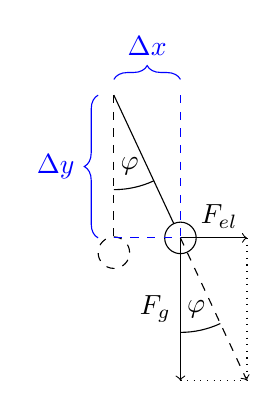
\begin{tikzpicture}
  \coordinate (mid) at (0,0); 
  \path (mid) ++({2*sin(155)}, {2*cos(155)}) coordinate (ball);
  \path (ball) ++({-0.2*sin(155)}, {-0.2*cos(155)}) coordinate (endline);
  \path (mid) ++(0, -2) coordinate (hypball);
  \path (hypball) ++(0, 0.2) coordinate (hypendline);
  \path (ball) ++({2*sin(155)}, 0) coordinate (endfel);
  \path (ball) ++(0, {2*cos(155)}) coordinate (endfg);
  \path (ball) ++({2*sin(155)}, {2*cos(155)}) coordinate (endf);
 
  \draw (mid) -- (endline);
  \draw (ball) circle (0.2);   
  \draw[dashed] (mid) -- (hypendline);
  \draw[dashed] (hypball) circle (0.2);
  \draw (0, -1.2) arc[start angle=-90, end angle=-65, radius=1.2];
  \draw (0.2, -0.9) node {$\varphi$}; 
  \draw[->] (ball) -- (endfel) node[midway, above, xshift=2pt] {$F_{el}$};
  \draw[->] (ball) -- (endfg) node[midway, left] {$F_{g}$};
 
  \draw[dashed, ->] (ball) -- (endf); 
  \draw[dotted] (endfel) -- (endf);
  \draw[dotted] (endfg) -- (endf);
  \draw (ball) ++ (0, -1.2) arc[start angle=-90, end angle=-65, radius=1.2];
  \draw (ball) ++ (0.2, -0.9) node {$\varphi$}; 
   
  \draw [blue, decorate,decoration={brace,amplitude=5pt}]
  (0, 0.2) -- ({2*sin(155)}, 0.2) node[midway,above, yshift=5pt]{$\Delta x$}; 
  \draw [blue, decorate,decoration={brace,amplitude=5pt,mirror}]
  (-0.2, 0) -- (-0.2, {2*cos(155)}) node[midway,left, xshift=-5pt]{$\Delta y$};
  \draw[blue, dashed] ({2*sin(155)}, 0) -- (ball);
  \draw[blue, dashed] (0, {2*cos(155)}) -- (ball);
 \end{tikzpicture} 
\end{minipage} 
 
\end{document}